%!TEX root = thesis.tex
\section{Concept}
\section{Related work}
\subsection{Electronic Textiles}
\begin{quotation}
\emph{The most profound technologies are those that disappear. They weave themselves into the fabric of everyday life until they are indistinguishable from it. \citep{weiser1991computer}}
\end{quotation}
One of the research areas that have stemmed from ubiquitous computing is electronic textiles or `e-textiles', which seeks to integrate electronic and computation into fabric.
\citet{park2002wearable} presents the E-Textile vision as the paradigm the ``fabric is the computer'', taking Weiser's much quoted description of ubiquitous computing very literal. 
E-textile is often used as part of wearable computing systems, logically, since clothing as a medium is ever present when people are invlolved.
\begin{figure}
\centering
\begin{minipage}[t]{.3\textwidth}
  \centering
  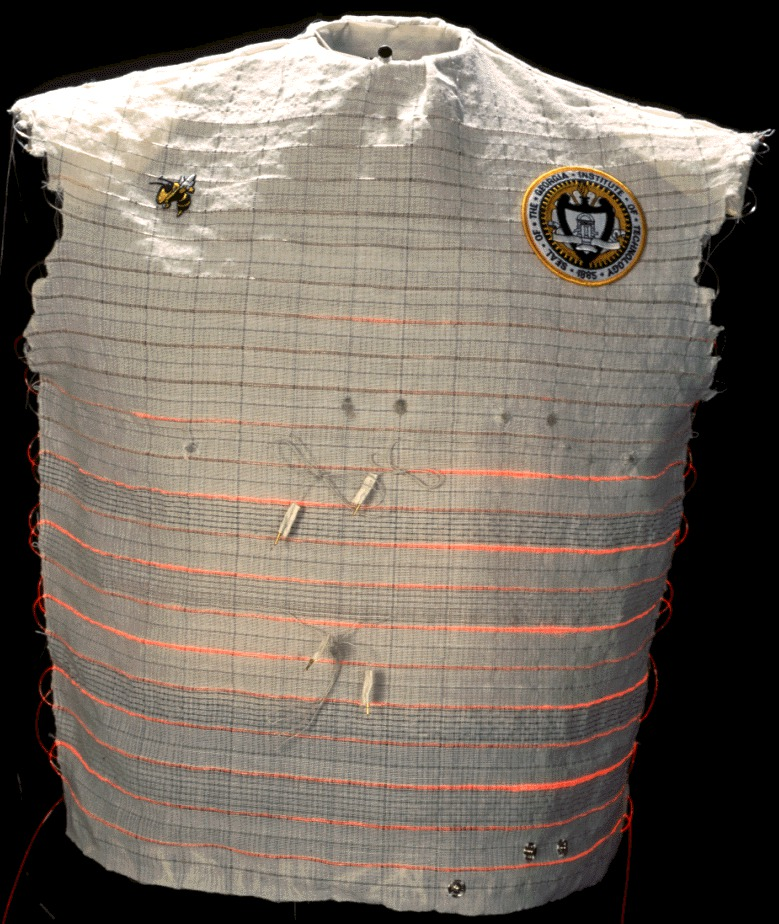
\includegraphics[width=0.8\linewidth]{figures/wearable_motherboard}
  \captionof{figure}{The Wearable Motherboard, taken from \citep{gopalsamy1999wearable}}
  \label{sofa_interaction:wearable_motherboard}
\end{minipage}%
\hspace{0.2cm}
\begin{minipage}[t]{.3\textwidth}
  \centering
  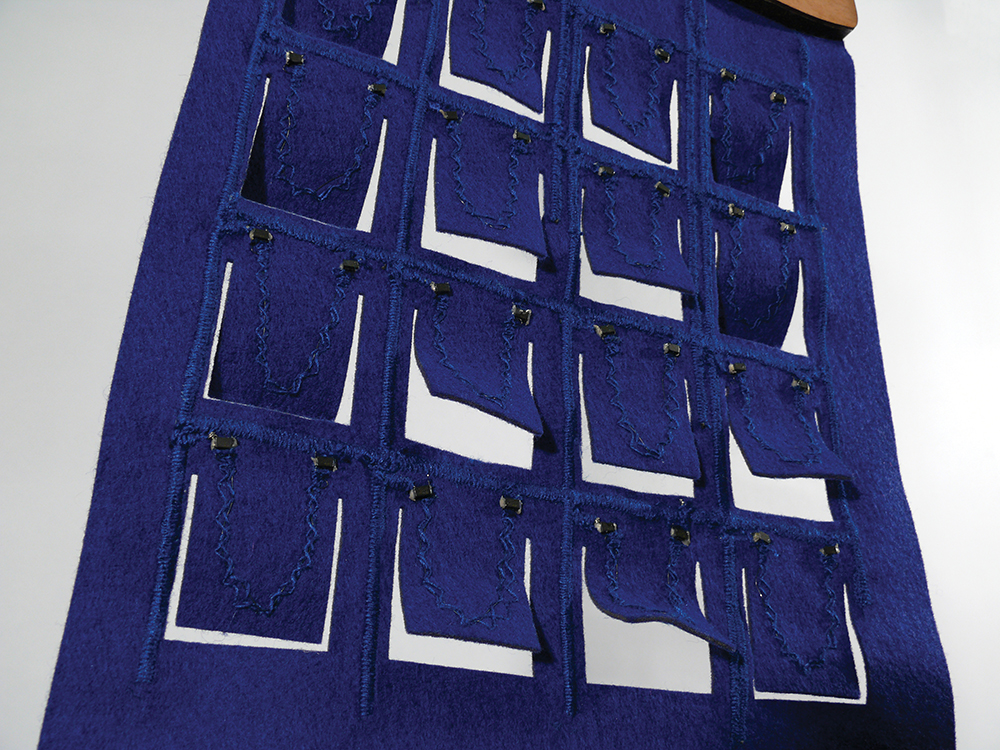
\includegraphics[width=0.8\linewidth]{figures/shutters}
  \captionof{figure}{Shutters, taken from \citep{coelho2009shutters}}
  \label{sofa_interaction:shutters}
\end{minipage}
\hspace{0.2cm}
\begin{minipage}[t]{.3\textwidth}
  \centering
  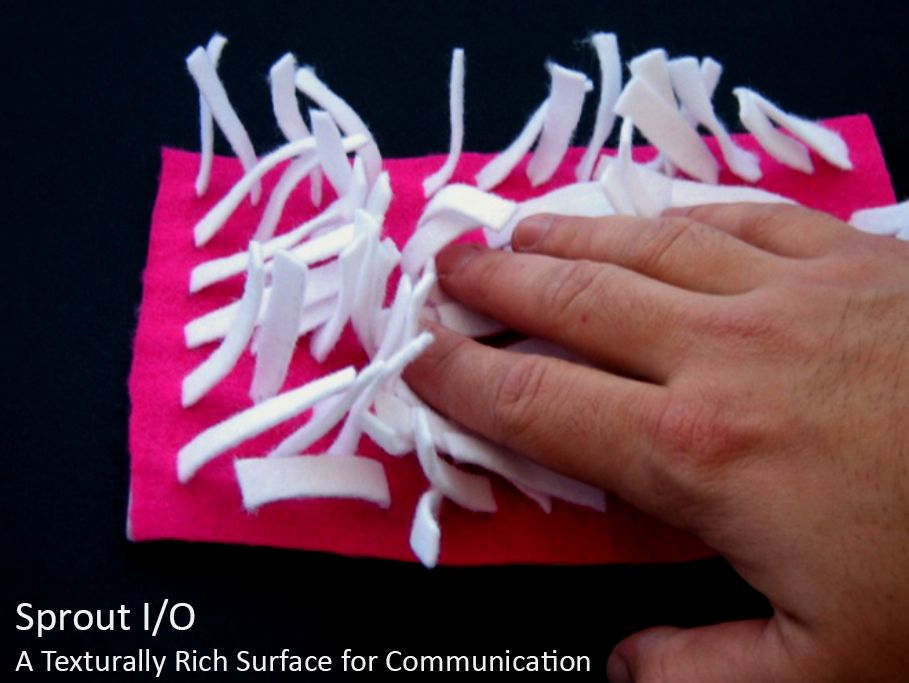
\includegraphics[width=0.8\linewidth]{figures/sprout}
  \captionof{figure}{Sprout I/O, taken from \citep{coelho2009shutters}}
  \label{sofa_interaction:sprout}
\end{minipage}
\end{figure}
A good example of this is the Wearable Motherboard \citep{gopalsamy1999wearable} seen in figure~\ref{sofa_interaction:wearable_motherboard}, also called the ``Smart Shirt'', which is a lightweight monitoring `jacket' that can provide sensory data for use in medical and military contexts.

E-textiles are not limited to wearable computing and clothing and can just as well be curtains, pillows, carpets, upholstery ect.
Shutters by \citet{coelho2009shutters}, seen in figure~\ref{sofa_interaction:shutters}, is an example of this where shape-memory alloy (SMA) threads are woven into a felt surface creating a curtain-like structure capable change of shape in permeability, used for indoor ventilation control among other things. 
Another example from \citet{coelho2008sprout} is Sprout I/O, see figure~\ref{sofa_interaction:sprout}, where a membrane filled with strands of SMA and felt provides textually rich input and actuated output capabilities.
By measuring the capacitance between the users hand and the individual SMA threads touches can be registered.


\begin{verbatim}
- DIY inspiration Plausea (rSkin)
- Leach Buechley
- Touch-matrix tekster
- $N recognition
\end{verbatim}
\section{Technicalities}
\section{Evaluation}